\documentclass{standalone}
\usepackage{tikz, pgfplots}
\pgfplotsset{compat=1.18}
\begin{document}
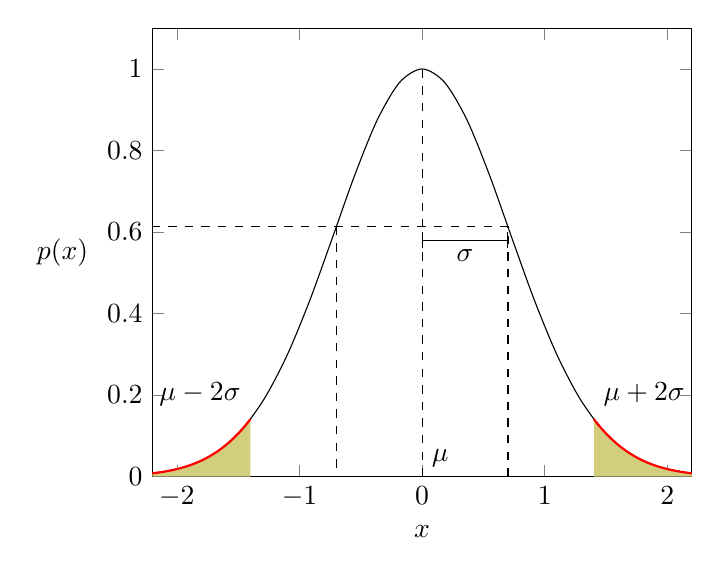
\begin{tikzpicture}
\begin{axis}[
    xlabel=$x$,
    ylabel=$p(x)$,
    ymin=0, 
    xmin=-2.2,xmax=2.2,
    ylabel style={rotate=-90},
    ]
    \addplot[smooth, domain=-2.2:2.2]
        {exp(-x^2)};
    \draw[dashed]
        (0,0)node[above right]{$\mu$}--(0,1)
        (0.7,0)--(0.7,0.6127)--(0,0.6127)--(-2.2,0.6127)
        (-0.7,0.6127)--(-0.7,0)
    ;
    \draw[|-|](0,0.58)--(0.7,0.58)node[midway, below]{$\sigma$};
    \addplot[draw=none, domain=-2.2:-1.4, fill=olive!40]{exp(-x^2)}\closedcycle;
    \addplot[draw=none, domain=2.2:1.4, fill=olive!40]{exp(-x^2)}\closedcycle;
    \addplot[solid, thick, red, domain=-2.2:-1.4]{exp(-x^2)};
    \addplot[solid, thick, red, domain=2.2:1.4]{exp(-x^2)};
    \draw
        (-1.4,0.15)node[above left]{$\mu-2\sigma$}
        (1.4,0.15)node[above right]{$\mu+2\sigma$}
    ;
\end{axis}
\end{tikzpicture}
\end{document}